\subsubsection{X-Axis: Horizontal Duplication}

The x-axis of the cube of the scalability is concerned with the horizontal
duplication and cloning of services and data with absolutely no bias, running
each identical copy of the system on a different server. Usually, the work is
distributed by a load balancer.

Reasoning on the x-axis is typically easy and the implementation can be fast,
but the data sets have to be replicated in their entirety which increases
operational costs.

% descrivere un esempio virtuoso fuori dall'architettura di Ethereum
In order to better understand the concept, we bring an example of a common
architecture which scales on this axis. Suppose you are running your own
e-commerce startup of wine. The business is going great and suddenly you have to
face the explosive growth of HTTP requests to your server. Since you have an
early stage startup, so far you had only a single server running on a single
machine, but you know that, if everything goes as hoped, you cannot scale-up for
a long time. So, you decide to take you Web server codebase and deploy an
identical copy of it. Right after, you set up
nginx\footnote{\url{http://nginx.org/}} as HTTP load balancer. The two Web
servers now work in parallel and access the same database, thanks to your
ability to write \emph{stateless} servers. The statelessness is an important
property in this scenario, it avoids dependency between requests, that is the
server can process a request without needing to access the information of
another one. In the example, if you would not have written a stateless server
(i.e. stateful), one request arrived at one of the two servers could be the ones
on which another request being processing on the other server depends on, hence
without permitting to successfully fulfill the latter.

\begin{figure}
  \centering
  \begin{subfigure}[m]{.4\textwidth}
    \centering
    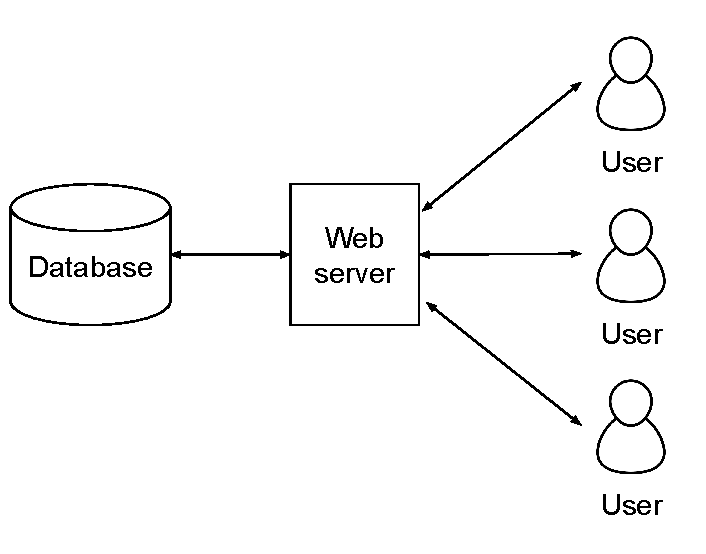
\includegraphics[height=4cm]{./res/img/webserver.pdf}
    \caption{}
    \label{fig:webserver}
  \end{subfigure}
  \hskip 3em
  \begin{subfigure}[m]{.4\textwidth}
    \centering
    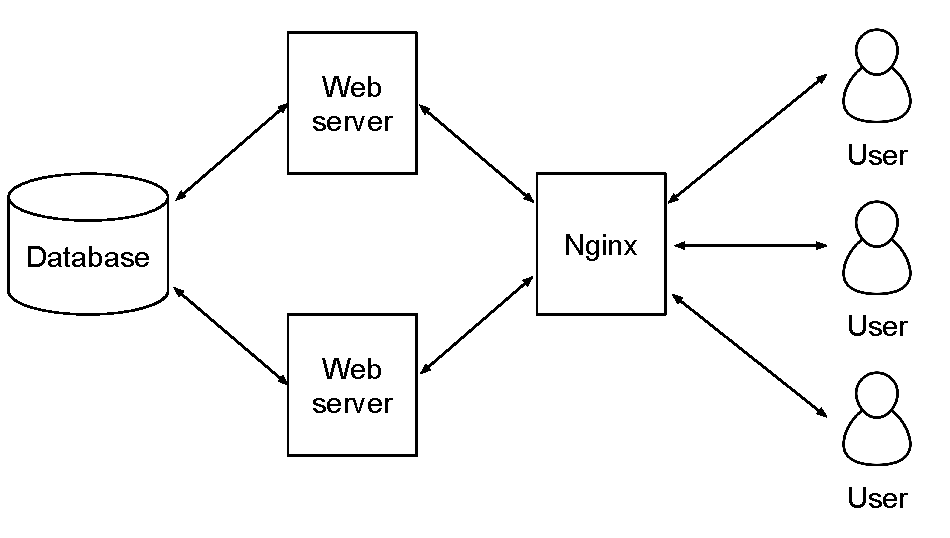
\includegraphics[height=4cm]{./res/img/webserver-nginx.pdf}
    \caption{}
    \label{fig:webserver-nginx}
  \end{subfigure}
  \caption{Web servers without (\protect\subref{fig:webserver}) and with (\protect\subref{fig:webserver-nginx}) load balancer.}
  \label{fig:webserver-scale-x}
\end{figure}

\paragraph{State}
Let's clarify the concept of \emph{state} in order to better understand the
importance of it scaling on the x-axis. We said that, in other words, an
application that uses state chooses the next action to be performed evaluating
the current execution condition \cite{bib:art-of-scalability}. This definition
holds for the protocols as well. A common example of stateless protocol is HTTP,
since it does not need to know anything about a previous request having all the
information needed to fulfill the current request. On the contrary, an example
of stateful application is a possible implementation of user session (which can
be done also with a stateless approach), in which a user is authorized to
request some resources only after an authentication request. In this setting,
the result of the authentication could be stored in the server making it
stateful, i.e. some requests are dependent on the authentication request.
Referring at \autoref{fig:webserver-nginx}, in the stateful implementation, the
user sessions could be stored at Web server level forcing them to communicate
with each other to check for open user sessions.
% add comparison between this state and the Ethereum state

It should be clear now the role of the \emph{state} scaling on the x-axis. Once
we scale by cloning, we duplicate the data along with the service. This can be
not a drawback at first, but it may become an issue increasing the data size.

\paragraph{Ethereum}
In \autoref{sec:background}, we already said that Ethereum is stateful, thus
making it difficult to scale on the x-axis. As we discussed in
\autoref{sec:network-layer}, the Ethereum implementation uses a peer-to-peer
network in which the nodes are \emph{servent}. Although there are different
clients (e.g. Geth\footnote{\url{https://github.com/ethereum/go-ethereum}},
Parity\footnote{\url{https://github.com/paritytech/parity}},
cpp-ethereum\footnote{\url{https://github.com/ethereum/cpp-ethereum}},
pyethapp\footnote{\url{https://github.com/ethereum/pyethapp}}, ecc.), each one
is compliant with the Ethereum protocols abstracting from the distinct
implementations, so this is not a distinctive characteristic from a functional
perspective. Let's not consider initially the possible different node types
\todo{Here we should discuss the different node types (full, archive, light) or
refer to a section} supposing that it can access the state and that it has its
own copy of it. In \autoref{sec:consensus:algorithm}, we introduced the Ethereum
consensus algorithm and the PoW algorithm which is run by the miners in order to
create the next valid block. The more miners join the network, thus incrementing
the global hash rate, the more difficult a state transition become, hence
duplicating the miners in the network does not increment the transaction
throughput making the scaling on the x-axis absent in the current
implementation.



% discutere sui mining pool

% discutere su Infura